\chapter{统计}

\section{基本概念}

\section{抽样}
\subsection{分层随机抽样}
\subsection{系统随机抽样}

\section{统计图表}
\subsection{频率分布直方图}
\begin{figure}[htb]
	\centering
	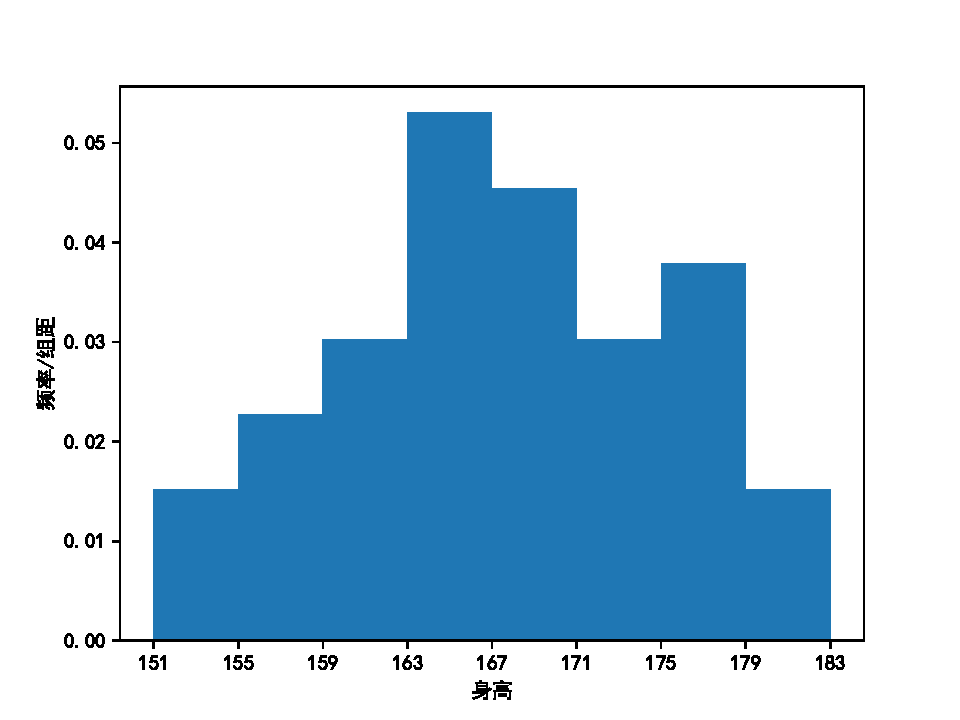
\includegraphics[width=0.6\linewidth]{src/images/chart1.pdf}
	\caption{身高的频率分布直方图}
	\label{fig:histogram}
\end{figure}

\subsection{频率分布折线图}
\begin{figure}[htb]
	\centering
	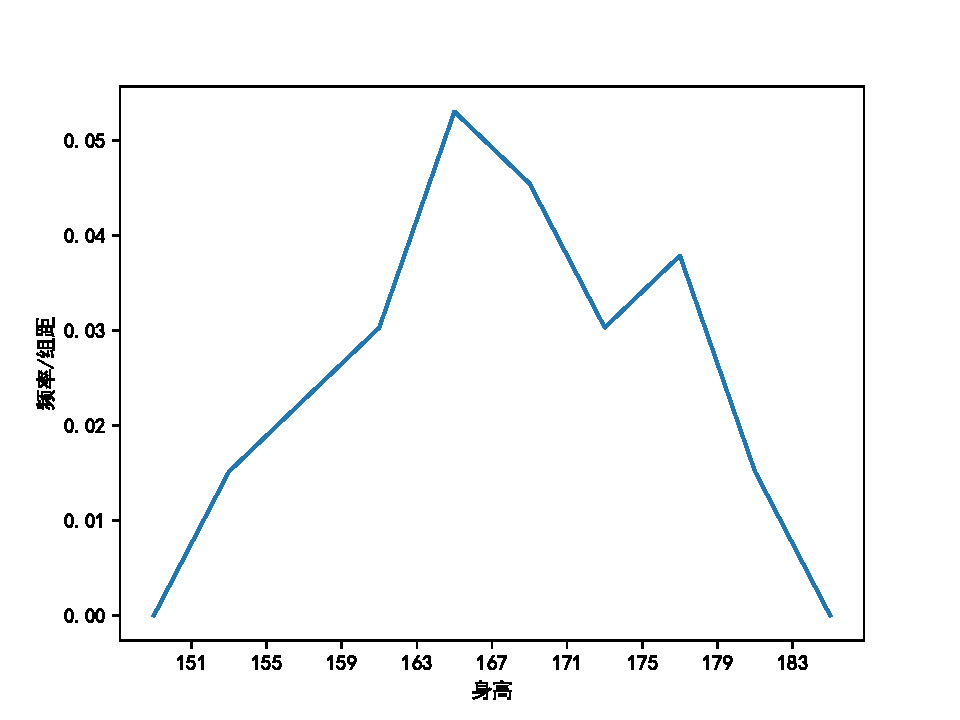
\includegraphics[width=0.6\linewidth]{src/images/chart2.pdf}
	\caption{身高的频率分布折线图}
	\label{fig:line-chart}
\end{figure}

\subsection{茎叶图}
\subsection{散点图}

\section{统计量}
在之前,我们已经学过了用均值和方差等统计量来估计总体的数字特征。现在,我们将复习已学的统计量并引入新的统计量。

\subsection{均值}
由于要表示大量数据的加法,我们引入求和符号$\Sigma$(读作sigma),${\displaystyle\sum_{i=1}^n a_i}$表示数列$a$从下标$i=1$到$i=n$的累加。

故此,均值公式可表示为
\begin{gather}
	\bar{x}=\frac{1}{n}\sum_{i=0}^n x_i \label{equ:mean-1}
\end{gather}

同时,当数据量很大且重复率高的情况下,有
\begin{gather}
	\bar{x}=\frac{1}{n}\sum_{i=0}^k x_if_i \label{equ:mean-2}
\end{gather}
其中$f_i$是$x_i$的频数(或者叫“权重”)。

\subsection{方差和标准差}
在初中我们已经知道了这两个统计量描述的是数据的离散程度,数据越离散,那么这组数据的方差和标准差就越大。

我们同样使用求和符号来表示\textbf{方差}(variance)
\begin{gather}
	s^2=\frac{1}{n}\sum_{i=0}^{n} (x_i-\bar{x})^2 \label{equ:variance}
\end{gather}

\textbf{标准差}(standard deviation)是方差算数平方根的结果
\begin{gather}
	s=\sqrt{\frac{1}{n}\sum_{i=0}^{n} (x_i-\bar{x})^2} \label{equ:standard-deviation}
\end{gather}

\subsection{百分位数}
一组数据的第$k$百分位数表示至少有$k\%$的数据小于或等于这个数,而同时也有$(100-k)\%$的数据大于或等于这个数。\textbf{百分位数}(percentile)也可用来描述数据的离散程度。

欲计算样本数为$n$的数据的第$k$百分位数$P_k$,先将其由小到大排列,并设$a=n\cdot k\%$。若$a$是整数,则$P_k$是第$a$项与第$a+1$项的均值;若$a$不是整数,那么$P_k$是第$\lceil a\rceil$项。

我们同时规定第25、50、75百分位数为\textbf{四分位数}。

\subsection{中位数和众数}
这两个统计量很简单,那就一笔带过吧。

\textbf{中位数}(median)是将数据项从小到大排列好后位于最中间的数。对于偶数个数据,则中位数不唯一,一般取最中间两数的均值。

\textbf{众数}(mode)是一组数据中出现频率最高的数,如果有多个数出现的频率最多,这意味着有多个众数。

\subsection{随机变量的分布特征}
我们使用一个2行的矩阵(也可以是表格)来表示随机变量的分布
\[\left(
	\begin{array}{cccc}
		x_1 & x_2 & \ldots & x_n \\
		p_1 & p_2 & \ldots & p_n \\
	\end{array}
\right)\]
